\documentclass[]{article}

%opening
\title{Exercises Set: Combinatorics}
\author{Paul Dubois}
\date{}

\usepackage{amsmath}
\usepackage{amsfonts}
\usepackage{amsthm}
\usepackage{amssymb}
\usepackage{mathrsfs}
\usepackage{stmaryrd}
\usepackage{graphicx}

\newcommand{\Q}{\mathbb{Q}}
\newcommand{\N}{\mathbb{N}}
\newcommand{\Z}{\mathbb{Z}}
\newcommand{\R}{\mathbb{R}}
\newcommand{\Primes}{\mathbb{P}}
\newcommand{\st}{\text{ s.t. }}
\newcommand{\txtand}{\text{ and }}
\newcommand{\txtor}{\text{ or }}
\newcommand{\lxor}{\veebar}


\begin{document}
	
	\maketitle
	
	\begin{center}
		\textit{Only the questions with a * are compulsory (but do all of them!).}
	\end{center}
	
	\section{Company employees *}
	\begin{center}
		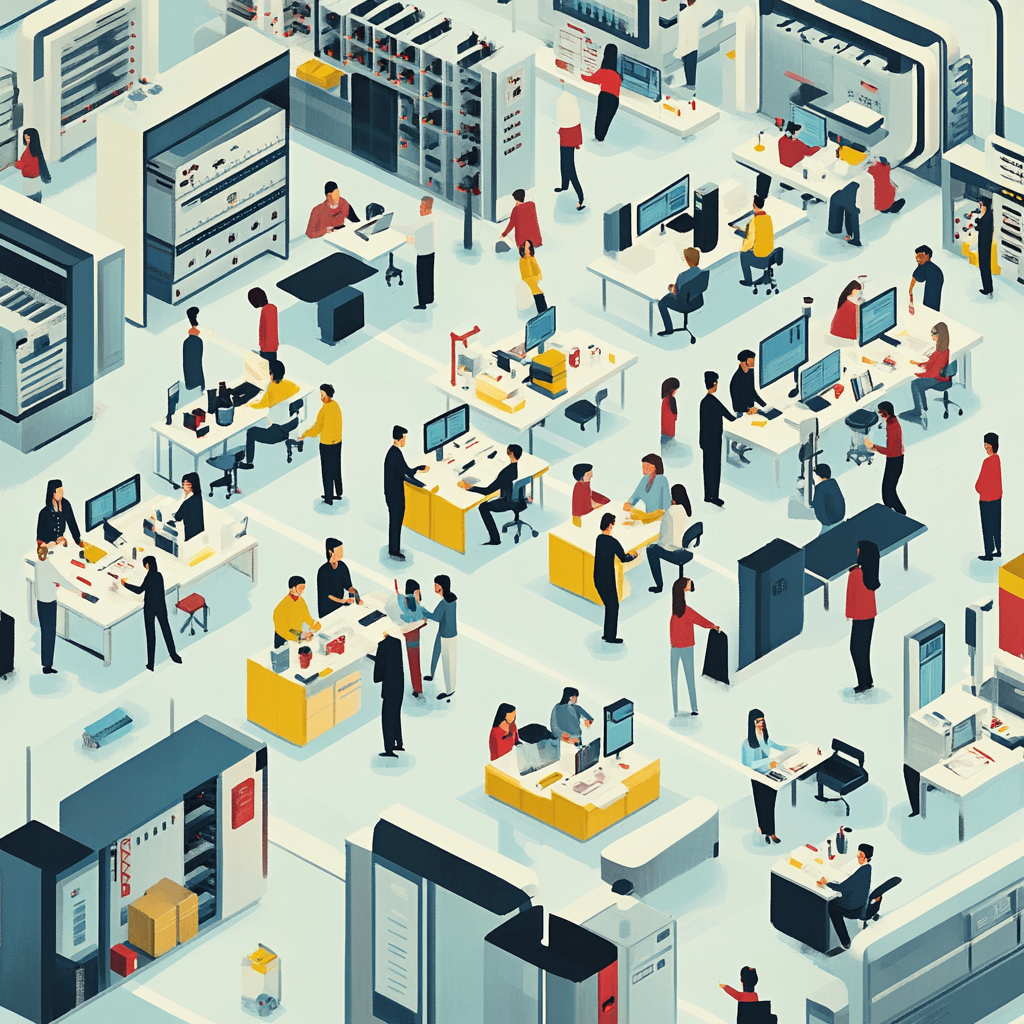
\includegraphics[height=8cm]{company.png}
	\end{center}
	In a company, there are 800 employees.\\
	300 are men, 352 are union members, 424 are married, 188 are union men, 166 are married men, 208 are union members and married, 144 are married union men.\\
	How many single, non-union women are there?
	
	\newpage
	\section{The padlock}
	\begin{center}
		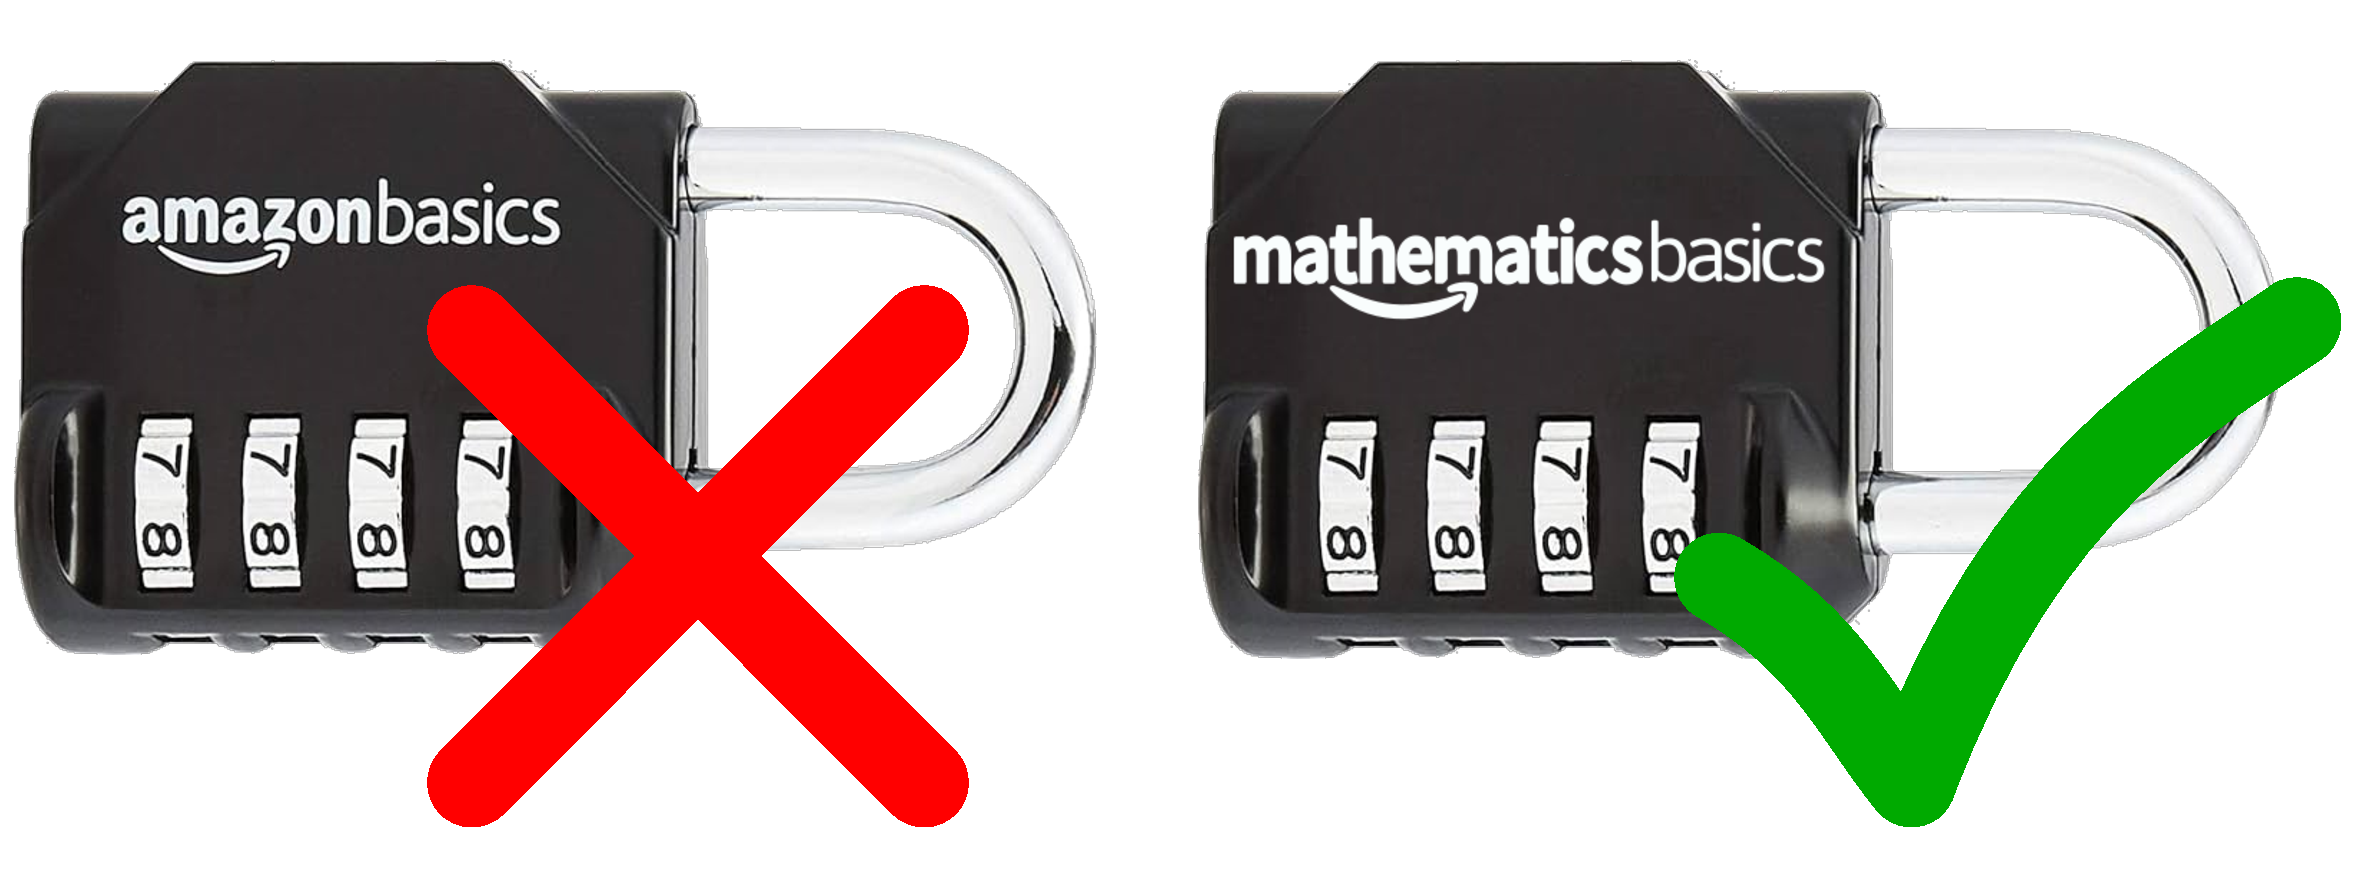
\includegraphics[width=12cm]{locks.pdf}
	\end{center}
	A padlock has a 4-digit code, each number being a number from 0 to 9.
	\begin{enumerate}
		\item How many possible codes are there?
		\item How many possible codes are there with 4 different digits?
		\item How many codes ending in an even number are there?
		\item How many codes are there ending with an even number and with 4 different numbers?
		\item How many codes are there containing at least one digit 4?
		\item How many codes are there containing exactly one digit 4?
	\end{enumerate}
	
	\newpage
	\section{Airplanes Company}
	\begin{center}
		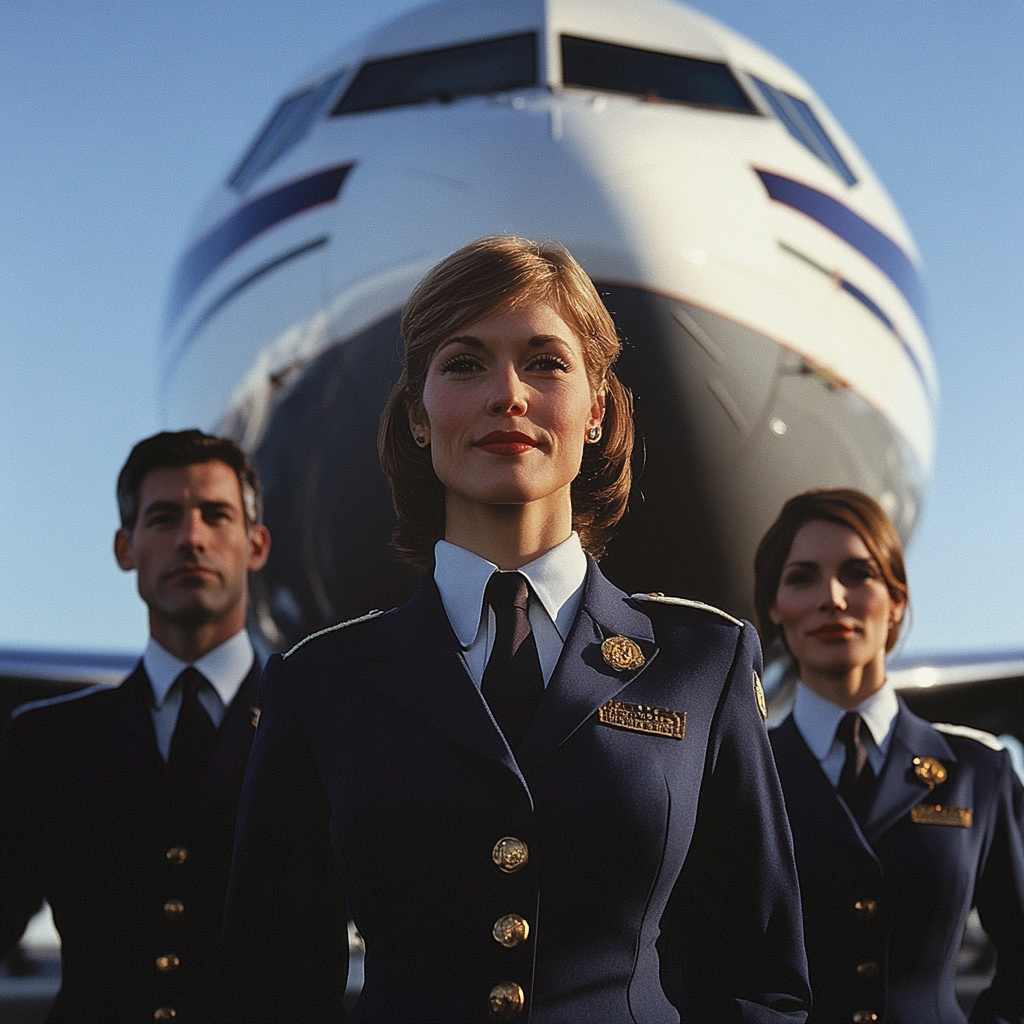
\includegraphics[width=5cm]{pilot_and_two_stewards_in_front_of_a_plane0.png}
		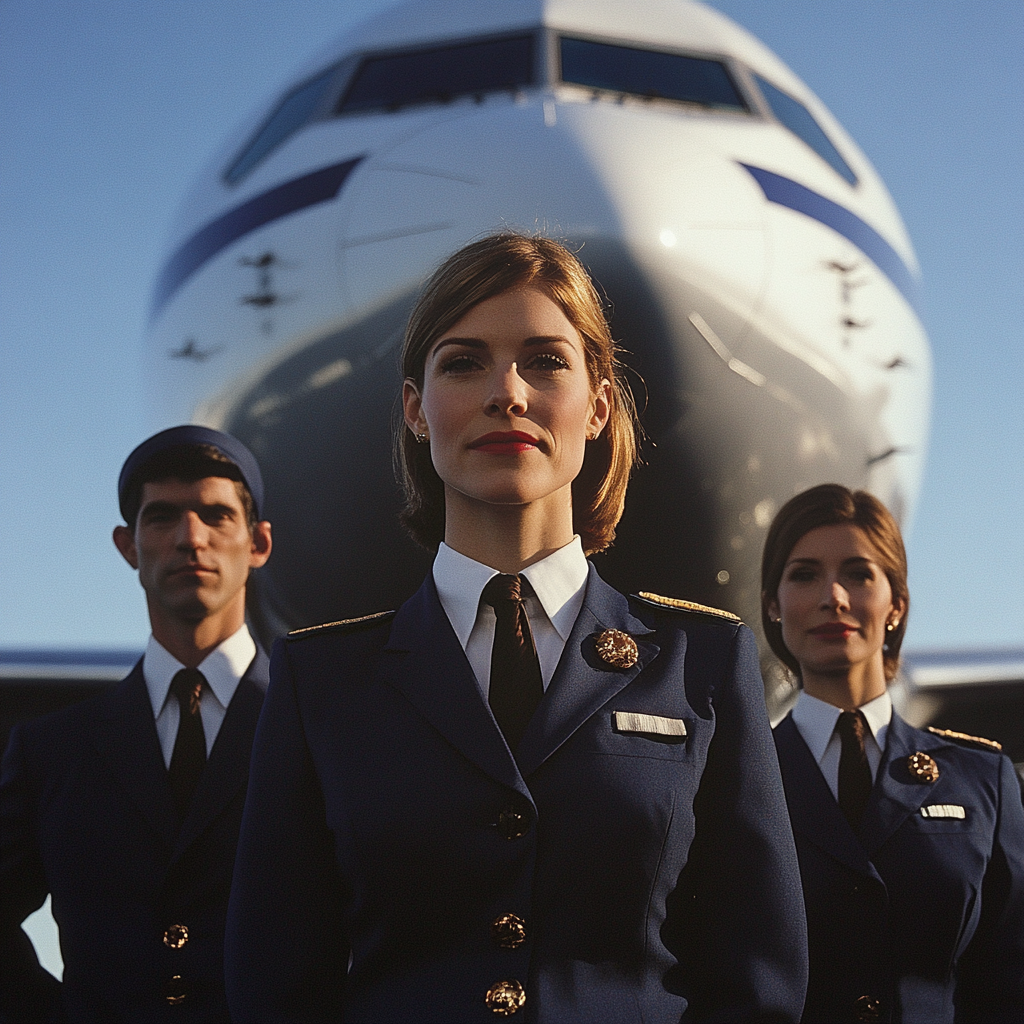
\includegraphics[width=5cm]{pilot_and_two_stewards_in_front_of_a_plane1.png}\\
		\vspace{0.8mm}
		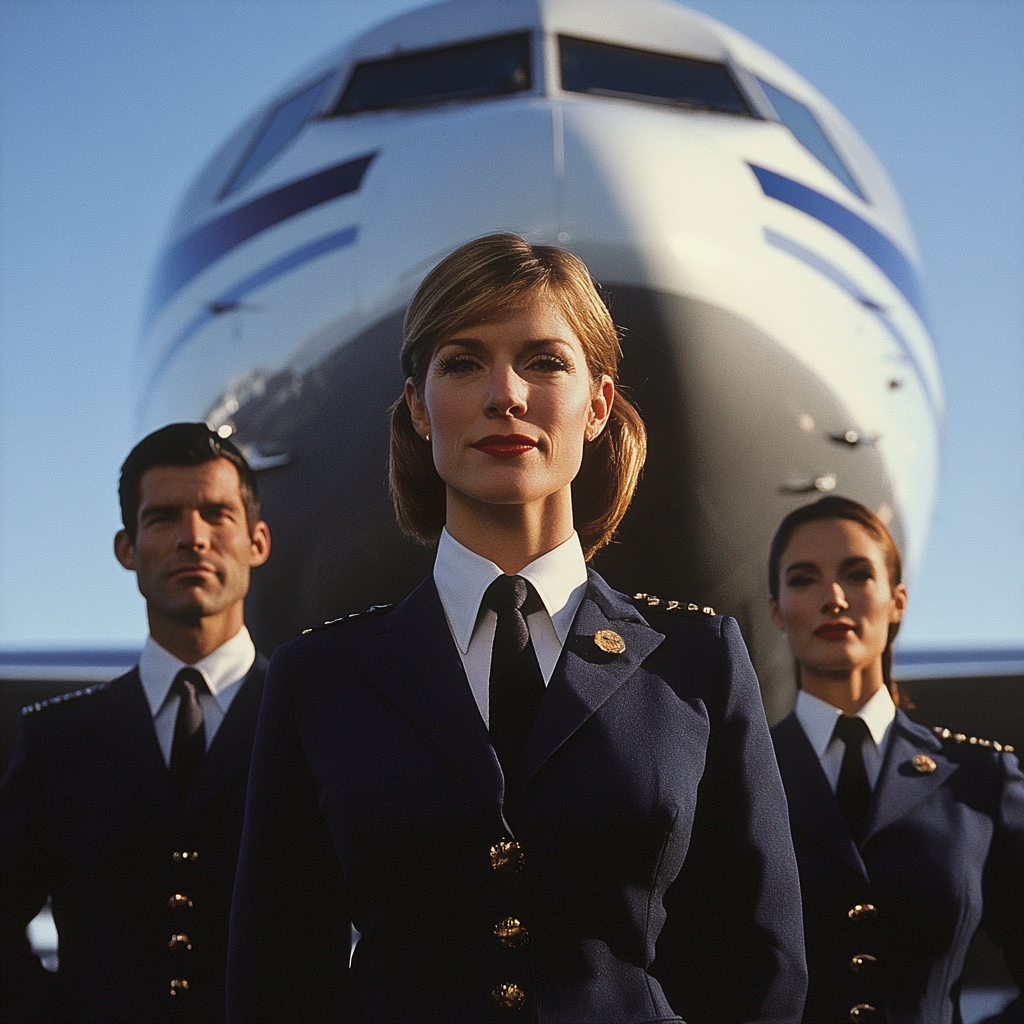
\includegraphics[width=5cm]{pilot_and_two_stewards_in_front_of_a_plane2.png}
		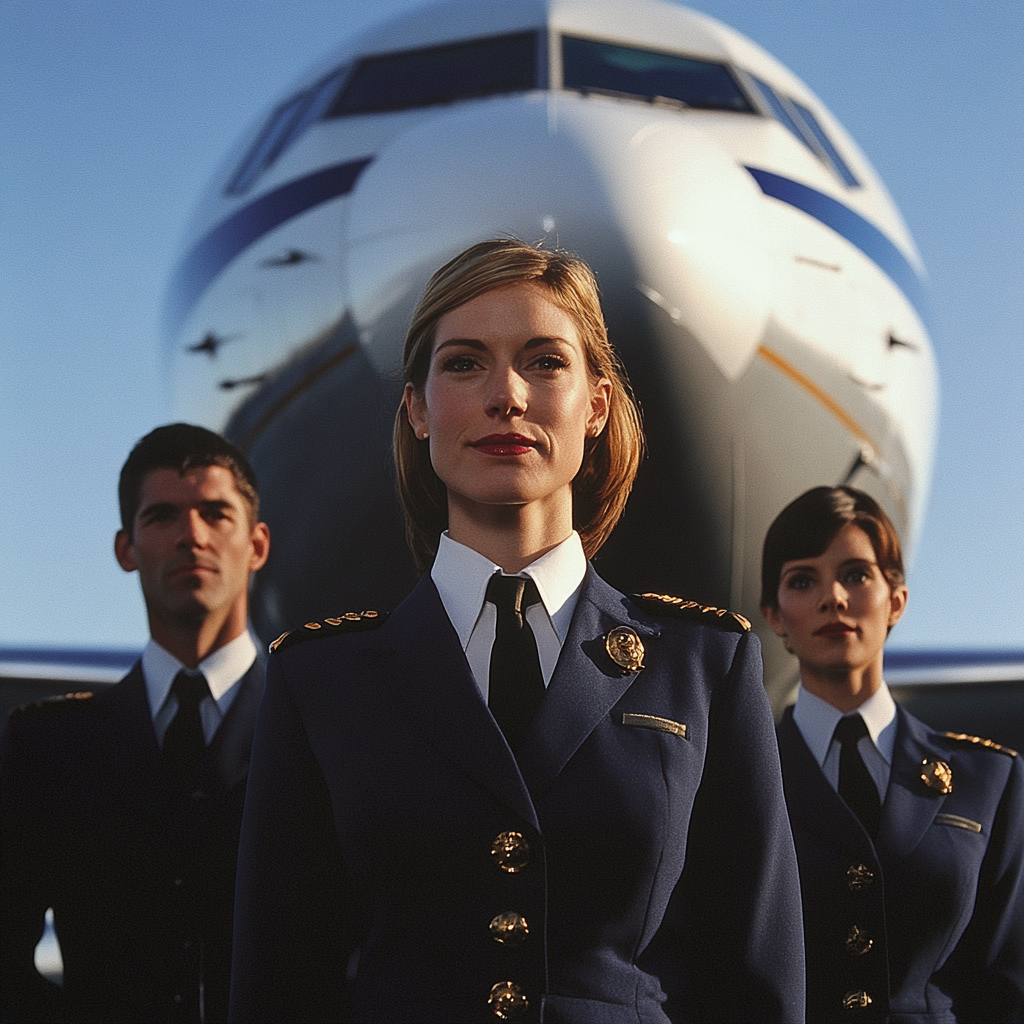
\includegraphics[width=5cm]{pilot_and_two_stewards_in_front_of_a_plane3.png}
	\end{center}
	A company has 4 airplanes, 4 pilots and 8 flight attendants.
	How many different ways are there to assign pilots and flight attendants to helicopters so that each helicopter has one pilot and two flight attendants?
	
	Explanations on the binomial coefficient.
	
	\newpage
	\section{Bookshelf *}
	\begin{center}
		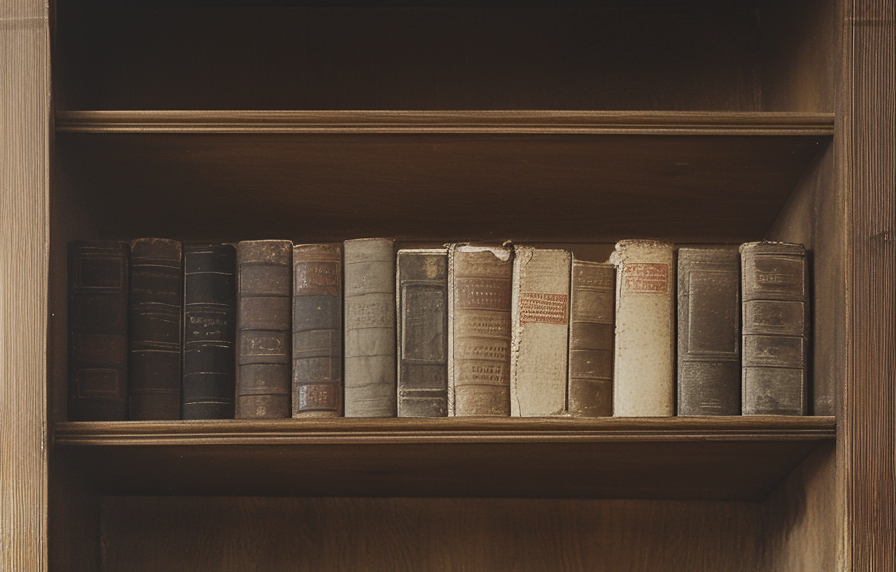
\includegraphics[width=10cm]{bookshelf.png}
	\end{center}
	We want to store 4 mathematics books (separate), 6 physics books, and 3 chemistry books on a shelf.
	How many ways can this storage be done:\\
	If books are to be grouped by subjects.\\
	If only math books should be grouped.
	
	\newpage
	\section{ESSEC's Stairs *}
	\begin{center}
		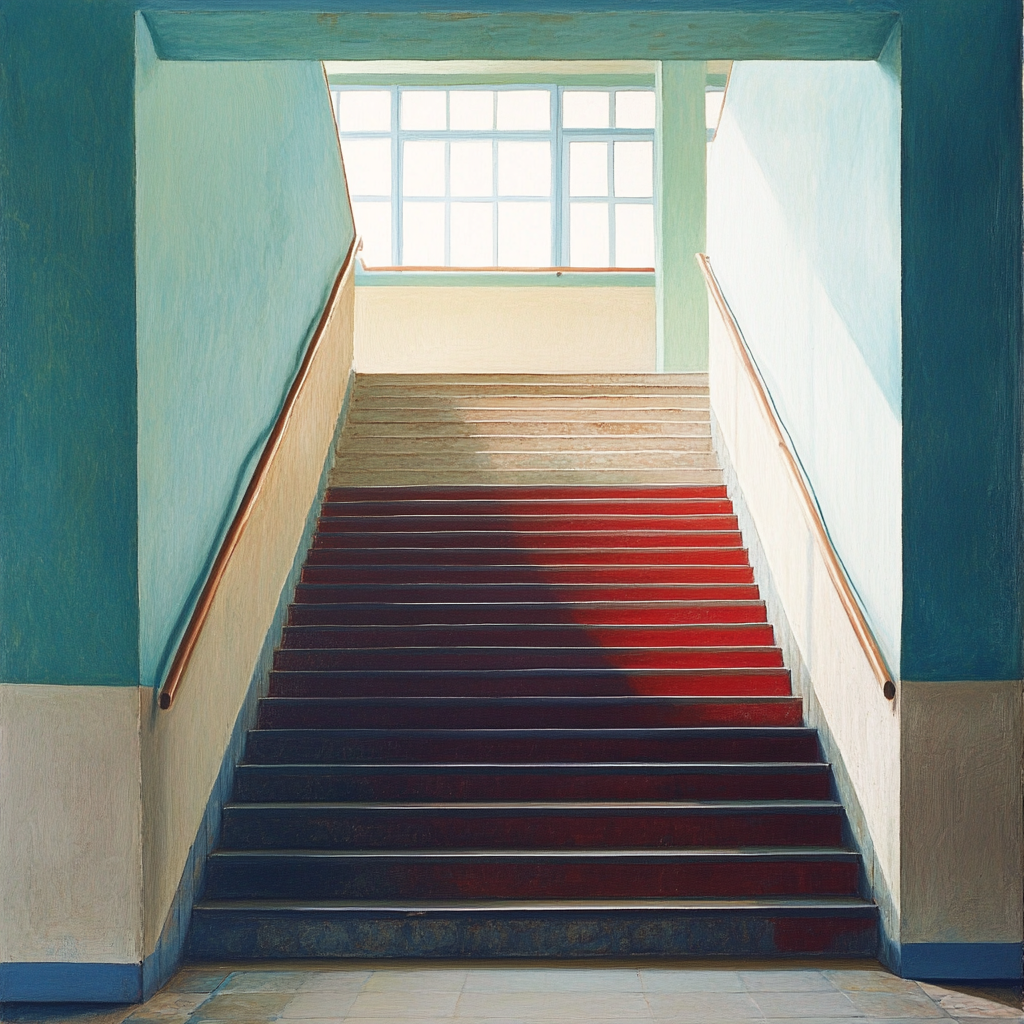
\includegraphics[height=8cm]{stairs.png}
	\end{center}
	At ESSEC, the staircase between the ground floor and the $1^{st}$ floor is made up of 16 steps.
	To climb this staircase, I can go up one step for each step, or up two steps. How many ways are there to climb this staircase?
	
	
	
	
\end{document}
